%! Author = gramic
%! Date = 21.03.24

% Preamble
\begin{flushleft}
%    \KOMAoptions{paper=A3,paper=landscape,DIV=20}
%\storeareas\landscapevaluesbig
    \begin{landscape}
        \subsection{Riskcontrolling}
        \subsubsection{Neu erfasste Risiken}
        \begin{table}[H]

\resizebox{\columnwidth}{!}{%

\begin{tabular}{rllllrrlrrl}
\toprule
ID & Definiert / Erkannt & Risiko & Beschreibung / Ursache & Auswirkung & WS & SM & Massnahmen notwendig & WS.1 & SM.1 & Massnahmen \\
\midrule
9 & \begin{tabular}[c]{@{}l@{}}19.03.2024\end{tabular} & \begin{tabular}[c]{@{}l@{}}Veeam Kasten K10\cite{P24LQGDK} nicht betriebsbereit\end{tabular} & Abhängigkeit zum KSGR k8s Projekt.\\Ohne Kubernetes kein Veeam Kasten. & \begin{tabular}[c]{@{}l@{}}Keine Kubernetes-Gerechten Sicherungen von Pods usw.\\Sicherungen Inkonsistent o.ä.\\Ohne Backup kann das Ziel des Projekts nicht erreicht werden\end{tabular} & 5 & 5 & Ja & 5 & 2 & \begin{tabular}[c]{@{}l@{}}Backup auf einem nfs-Share ablegen.\\So können Test-DBs wenigstens gesichert werden.\end{tabular} \\
\bottomrule
\end{tabular}
}
\caption{Neu Erkannte / Erfasste Risiken} \label{riskcontrolling_new_risks}
\end{table}

    \end{landscape}
\end{flushleft}
\begin{flushleft}
    \begin{landscape}
        \subsubsection{Assessment 21.03.2024}
        \begin{table}[H]

\resizebox{\columnwidth}{!}{%

\begin{tabular}{rllrrllll}
\toprule
ID & Risiko & Assessment-Datum & WS & SM & Dringlichkeit & Ergriffene Massnahmen & Wirksamkeit & Begründung \\
\midrule
1 & \begin{tabular}[c]{@{}l@{}}Fehlende Ressourcen\end{tabular} & 21.03.2024 & 3 & 4 & hoch & \begin{tabular}[c]{@{}l@{}}Dokumentation ausserhalb Arbeitszeit\end{tabular} & begrenzt & \begin{tabular}[c]{@{}l@{}}Mentale Ressourcen setzen Limits.\end{tabular} \\
2 & \begin{tabular}[c]{@{}l@{}}HP-UX Ablöseprojekt\end{tabular} & 21.03.2024 & 5 & 4 & sehr hoch & \begin{tabular}[c]{@{}l@{}}Ressourcen reserviert\end{tabular} & begrenzt & \begin{tabular}[c]{@{}l@{}}ExaCC Server werden mitten während der Diplomarbeit geliefert.\\Von KSGR Seite fehlt eine Stellvertretung.\\Mithilfe notwendig.\end{tabular} \\
3 & \begin{tabular}[c]{@{}l@{}}Alte Infrastruktur kann\\ungeplant sämtliche Ressourcen binden\end{tabular} & 21.03.2024 & 4 & 4 & hoch & \begin{tabular}[c]{@{}l@{}}Externe Partner sensibilisiert\end{tabular} & wirksam & \begin{tabular}[c]{@{}l@{}}Externe Partner können meinen Teil der Aufgaben  bei Problemen abfedern.\\Allerdings nicht vollständig\end{tabular} \\
4 & \begin{tabular}[c]{@{}l@{}}Schwächen beim\\Selbstmanagement\\und in der Selbstorganisation\end{tabular} & 21.03.2024 & 3 & 3 & hoch & \begin{tabular}[c]{@{}l@{}}- Projektplanung erstellt.\\- Arbeitspakete geplant\end{tabular} & begrenzt & \begin{tabular}[c]{@{}l@{}}Nicht an alle Tasks gedacht, wie z.B. Risikocontrolling.\end{tabular} \\
5 & \begin{tabular}[c]{@{}l@{}}Scope Verlust während des Projekts\end{tabular} & 21.03.2024 & 2 & 2 & mittel & \begin{tabular}[c]{@{}l@{}}Ziele SMART definiert\end{tabular} & wirksam & \begin{tabular}[c]{@{}l@{}}Ziele sind klar definiert.\\Allerdings gibt es zwangsweise gewisse Unschärfen.\end{tabular} \\
6 & \begin{tabular}[c]{@{}l@{}}Scope Creep\end{tabular} & 21.03.2024 & 3 & 3 & hoch & \begin{tabular}[c]{@{}l@{}}Ziele SMART definiert\end{tabular} & gebrenzt & \begin{tabular}[c]{@{}l@{}}Sehr viele mögliche Lösungen am Markt.\end{tabular} \\
7 & \begin{tabular}[c]{@{}l@{}}SIEM / Log Plattform\\nicht betriebsbereit\end{tabular} & 21.03.2024 & 5 & 1 & sehr hoch & \begin{tabular}[c]{@{}l@{}}keine\end{tabular} &  & \begin{tabular}[c]{@{}l@{}}SIEM wird nicht rechtzeitig stehen.\\Das Schadensmass ist aber zu gering,\\damit Massnahmen ergriffen werden müssten.\end{tabular} \\
8 & \begin{tabular}[c]{@{}l@{}}Foreman nicht betriebsbereit\end{tabular} & 21.03.2024 & 1 & 1 & erledigt & \begin{tabular}[c]{@{}l@{}}keine\end{tabular} &  & \begin{tabular}[c]{@{}l@{}}Foreman ist in Betrieb\end{tabular} \\
9 & \begin{tabular}[c]{@{}l@{}}Veeam Kasten K10\cite{P24LQGDK} nicht betriebsbereit\end{tabular} & 21.03.2024 & 5 & 5 & sehr hoch & \begin{tabular}[c]{@{}l@{}}noch keine\end{tabular} &  & \begin{tabular}[c]{@{}l@{}}\end{tabular} \\
\bottomrule
\end{tabular}
}
\caption{Risiko-Assessment 21.03.2024} \label{risk_assessments_21_03_2024}
\end{table}

    \end{landscape}
    \begin{figure}[H]
        \centering
        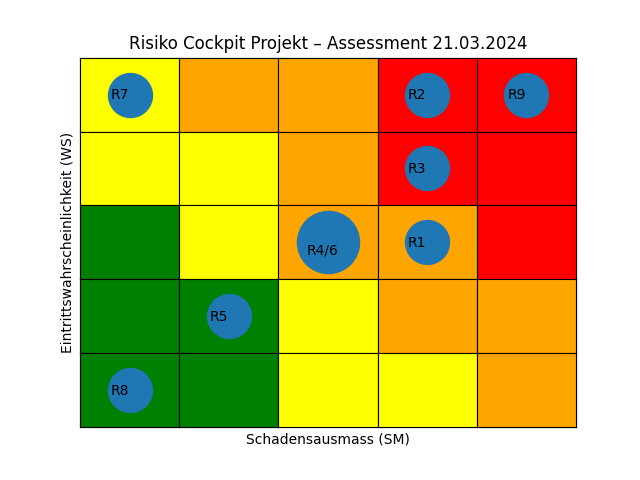
\includegraphics[width=0.75\linewidth]{source/riskmatrix/project-assessment-21-03-2024}
        \caption{Riskikomatrix - Assessment 21.03.2024}
        \label{fig:project-assessment-21-03-2024}
    \end{figure}
\end{flushleft}